\section{Results}\label{sec:results}

\subsection{Reproduction of TCPDBench}
Table~\ref{tab:tcpdbench} compares our default-setting baselines with the scores stored by TCPDBench on the 32 univariate TCPD series. For Zero, Binary Segmentation and BOCPD, F1 and covering match to three decimals. PELT returns the same change points as the R \texttt{changepoint} run on every series. Its covering also matches (0.652). Its F1 is lower (0.657 vs.\ 0.674) only because TCPDBench stores each PELT change point one index early. Our metrics and baselines therefore reproduce the published benchmark, and the TSFM detectors below are scored on exactly the same footing.

\begin{table}[t]
\centering
\caption{Mean F1 (margin 5) and segmentation covering over series. Default: fixed parameters; oracle: best of each method's grid per series.}
\label{tab:main}
\resizebox{\columnwidth}{!}{%
\begin{tabular}{lrrrrrrrr}
\toprule
Method & TCPD default F1 & TCPD default Cov & TCPD oracle F1 & TCPD oracle Cov & SKAB default F1 & SKAB default Cov & SKAB oracle F1 & SKAB oracle Cov \\
\midrule
Zero (no CPs) & 0.638 & 0.554 & 0.638 & 0.554 & 0.349 & 0.364 & 0.349 & 0.364 \\
PELT & 0.652 & 0.640 & 0.864 & 0.772 & 0.147 & 0.248 & 0.512 & 0.754 \\
BinSeg & 0.686 & 0.665 & 0.861 & 0.774 & 0.347 & 0.621 & 0.463 & 0.727 \\
BOCPD & 0.656 & 0.578 & 0.892 & 0.785 & 0.185 & 0.369 & 0.559 & 0.699 \\
\bottomrule
\end{tabular}
}
\end{table}

\begin{table}[t]
\centering
\caption{Paired Wilcoxon signed-rank tests of per-series F1 against the best classical baseline of each dataset and setting (Holm-corrected over the three TSFM detectors).}
\label{tab:stats}
\resizebox{\columnwidth}{!}{%
\begin{tabular}{lrrrrrrr}
\toprule
Dataset & Setting & Detector & vs & Median diff & W/T/L & p & p (Holm) \\
\midrule
TCPD & default & Chronos-2 residual & BinSeg & -0.037 & 14/3/19 & 0.649 & 0.735 \\
TCPD & default & TimesFM-2.5 residual & BinSeg & -0.063 & 12/1/23 & 0.368 & 0.735 \\
TCPD & default & Chronos-2 embedding & BinSeg & -0.094 & 12/0/24 & 0.069 & 0.208 \\
TCPD & oracle & Chronos-2 residual & BOCPD & -0.038 & 9/6/21 & 0.006 & 0.012 \\
TCPD & oracle & TimesFM-2.5 residual & BOCPD & -0.033 & 11/5/20 & 0.016 & 0.016 \\
TCPD & oracle & Chronos-2 embedding & BOCPD & -0.132 & 5/7/24 & 0.000 & 0.000 \\
SKAB & default & Chronos-2 residual & BinSeg & -0.030 & 13/1/20 & 0.396 & 0.396 \\
SKAB & default & TimesFM-2.5 residual & BinSeg & -0.097 & 10/1/23 & 0.033 & 0.098 \\
SKAB & default & Chronos-2 embedding & BinSeg & 0.006 & 17/1/16 & 0.150 & 0.301 \\
SKAB & oracle & Chronos-2 residual & BOCPD & -0.119 & 4/5/25 & 0.000 & 0.000 \\
SKAB & oracle & TimesFM-2.5 residual & BOCPD & -0.213 & 1/7/26 & 0.000 & 0.000 \\
SKAB & oracle & Chronos-2 embedding & BOCPD & -0.238 & 5/3/26 & 0.000 & 0.000 \\
\bottomrule
\end{tabular}
}
\end{table}


\subsection{Default setting: zero-shot TSFMs vs.\ untuned classical CPD}
Table~\ref{tab:main} gives mean F1 and covering, and Fig.~\ref{fig:box} shows the per-series spread of F1 in the default setting.

\textbf{TCPD.} The Chronos-2 residual detector reaches a mean F1 of 0.668. It is second of the six detectors, behind Binary Segmentation (0.686) and ahead of BOCPD (0.656) and PELT (0.652). It also has the highest median per-series F1 of all methods (0.711). TimesFM-2.5 residual (0.641) is only just above Zero (0.638), and the embedding detector (0.605) falls below it. On covering, Binary Segmentation (0.665) and PELT (0.640) lead, ahead of Chronos-2 residual (0.608).

\textbf{SKAB.} No detector beats Zero under F1 (0.349). The best are Binary Segmentation (0.333) and Chronos-2 residual (0.303). Under covering, every detector except PELT scores above Zero (0.364). Binary Segmentation leads (0.616), followed by the embedding detector (0.575).

\textbf{Significance.} Binary Segmentation is the best classical method in the default setting on both datasets. Table~\ref{tab:stats} compares each TSFM detector with it. None of the three differs significantly from it on either dataset: all Holm-corrected $p\geq0.098$. On TCPD, Chronos-2 residual wins on 14 series, ties on 3 and loses on 19 (median difference $-0.037$, $p=0.735$). On SKAB, the embedding detector wins on slightly more series than it loses (17/1/16).

\begin{figure*}[t]
\centering
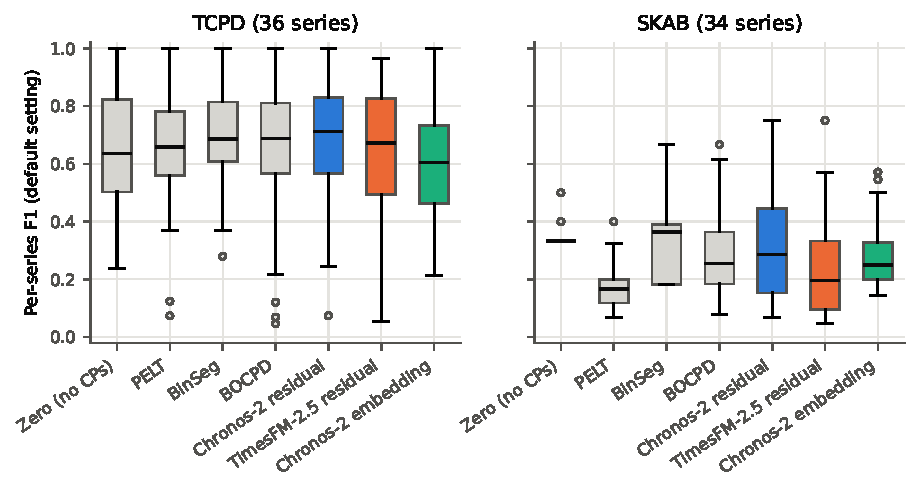
\includegraphics[width=0.85\textwidth]{fig3_f1_boxplot}
\caption{Per-series F1 in the default setting. TSFM detectors are coloured; classical methods and Zero are grey.}
\label{fig:box}
\end{figure*}

\subsection{Oracle setting}
Tuning per series raises every method, but the classical methods gain more (Table~\ref{tab:main}). BOCPD reaches 0.892 on TCPD, against 0.828 for Chronos-2 residual, 0.827 for TimesFM-2.5 residual and 0.739 for the embedding detector. On SKAB it reaches 0.634, against 0.477, 0.426 and 0.422. All six differences are significant after Holm correction: on TCPD $p=0.012$, $0.016$ and $<0.001$; on SKAB $p<0.001$ for all three (Table~\ref{tab:stats}).

The classical grids are larger (83--501 configurations against 40 for each residual detector), so we also cut every classical grid to 40 evenly spaced configurations. Oracle F1 drops only slightly:
\begin{itemize}
\item BOCPD: 0.871 on TCPD and 0.600 on SKAB;
\item PELT: 0.857 and 0.572;
\item Binary Segmentation: 0.855 and 0.526.
\end{itemize}
All of these remain above the best TSFM oracle (0.828 on TCPD, 0.477 on SKAB). The oracle gap is therefore not an artefact of grid size.

\subsection{Effect of series length}
We split the TCPD default F1 by series length into four groups:
\begin{itemize}
\item \emph{Shorter than 100 points (9 series).} BOCPD leads (0.833), followed by Chronos-2 residual (0.811) and TimesFM-2.5 residual (0.807). Both are well ahead of PELT and Binary Segmentation (0.727 each).
\item \emph{100--255 points (9 series).} Binary Segmentation (0.795) and PELT (0.758) lead, ahead of Chronos-2 residual (0.734) and TimesFM-2.5 residual (0.729).
\item \emph{256--511 points (10 series).} Chronos-2 residual is the best method (0.678), narrowly ahead of BOCPD (0.672) and PELT (0.671).
\item \emph{512 points or more (8 series).} Every detector falls below Zero (0.702). The lowest scores are TimesFM-2.5 residual (0.376), BOCPD (0.405) and Chronos-2 residual (0.421).
\end{itemize}
All SKAB files are longer than 512 points (745--1327).

\subsection{Context length and the first time steps}
Fig.~\ref{fig:context} shows mean F1 for each context length $L$ at the default $\tau=3$. On TCPD, F1 stays between 0.653 and 0.679 for Chronos-2 and between 0.639 and 0.668 for TimesFM-2.5. On SKAB, the longest context ($L=256$) is best for both models (0.322 and 0.281). The default $L=128$ was fixed in advance and is not the best on either dataset. The best $L$ would add 0.011 (Chronos-2) and 0.026 (TimesFM-2.5) to mean F1 on TCPD, and 0.019 and 0.038 on SKAB.

In its first steps, the residual detector forecasts from a very short context. To check whether this produces spurious detections, we set the scores of the first 32 steps to zero. SKAB F1 rises by less than 0.01 (0.303 to 0.308 for Chronos-2, 0.244 to 0.250 for TimesFM-2.5). TCPD F1 falls (0.668 to 0.627 and 0.641 to 0.618), because 15 of the 36 TCPD series have an annotated change point in their first 32 steps. The results are therefore not driven by an early-context artefact.

\begin{figure*}[t]
\centering
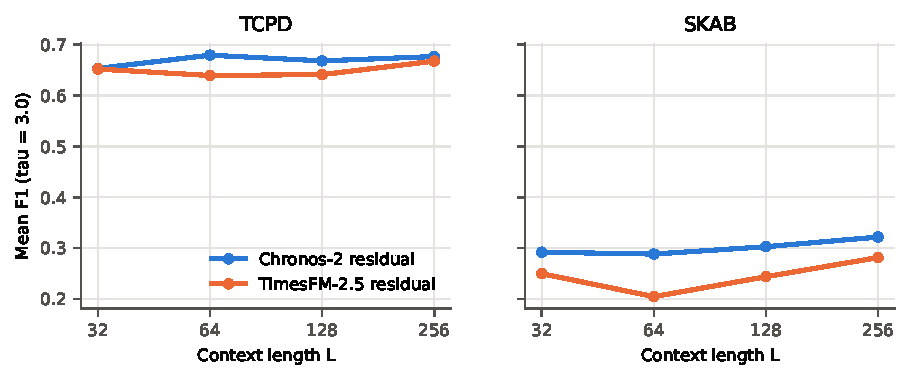
\includegraphics[width=0.85\textwidth]{fig4_context_length}
\caption{Mean F1 of the residual detectors against context length $L$ ($\tau=3$).}
\label{fig:context}
\end{figure*}

\begin{table}[t]
\centering
\caption{Mean runtime per series at default parameters. Classical methods: one CPU core; TSFM detectors: one Colab T4 GPU (model inference only).}
\label{tab:runtime}
\resizebox{\columnwidth}{!}{%
\begin{tabular}{lrr}
\toprule
Method & SKAB (s/series) & TCPD (s/series) \\
\midrule
BinSeg & 0.36 & 0.09 \\
BOCPD & 0.70 & 0.33 \\
Chronos-2 embedding & 6.59 & 0.30 \\
Chronos-2 residual & 11.41 & 0.51 \\
PELT & 2.91 & 0.49 \\
TimesFM-2.5 residual & 25.49 & 1.62 \\
\bottomrule
\end{tabular}
}
\end{table}


\subsection{Runtime}
Table~\ref{tab:runtime} reports the mean runtime per series in the default setting. On SKAB, the classical methods need 0.36\,s (Binary Segmentation), 0.70\,s (BOCPD) and 2.91\,s (PELT) on one CPU core. The TSFM detectors need 6.59\,s (embedding), 11.41\,s (Chronos-2 residual) and 25.49\,s (TimesFM-2.5 residual) on a T4 GPU, counting model inference only. The residual detector needs one forecast per time step. TimesFM-2.5 is the slowest, partly because it forecasts each of SKAB's 8 channels separately. The hardware differs, so these numbers show the order of magnitude rather than a like-for-like comparison.

\subsection{Qualitative example}
Fig.~\ref{fig:example} shows the TimesFM-2.5 residual score on two series. Both were chosen before any TSFM result was seen. On \texttt{nile}, the score peaks just after the annotated change, but the peak stays below $\tau=3$, so the default setting reports no change point. On \texttt{valve1\_0}, the score crosses $\tau$ many times away from the four annotated change points, including a very large spike in the first steps, where the context is shortest.

\begin{figure*}[t]
\centering
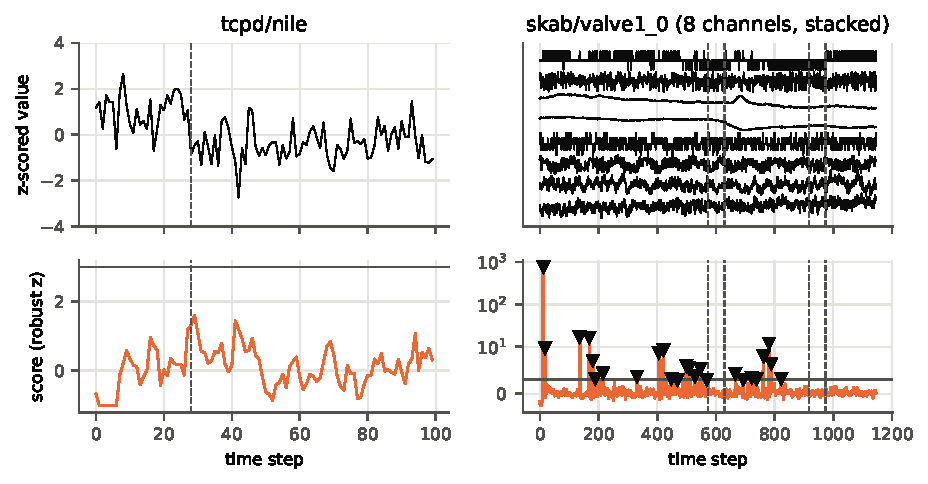
\includegraphics[width=0.85\textwidth]{fig2_example}
\caption{TimesFM-2.5 residual detector ($L=128$, $\tau=3$) on TCPD \texttt{nile} (left) and SKAB \texttt{valve1\_0} (right, 8 channels stacked). Top: z-scored series. Bottom: the standardised score that peak picking sees, with the threshold $\tau$ (solid line) and the detections (triangles). Dashed lines mark the annotated change points.}
\label{fig:example}
\end{figure*}

\section{Discussion}
\textbf{Answer to the research question.} Partly. With no training and no tuning, the Chronos-2 forecast residual locates change points about as well as untuned classical CPD on real-world data. It is statistically tied with the best classical method on TCPD and has the highest median F1 there. The observation of Uray et al.~\cite{uray2026exploring}, that forecast error spikes at changes, therefore holds up as a usable detector. It is not a replacement for classical CPD, though: once methods are tuned the classical ones are significantly better, and the TSFM detectors are weak on long series and on the industrial SKAB data.

\textbf{Where the TSFM detectors fail.} Fig.~\ref{fig:example} suggests a likely reason for the weak results on long and noisy multichannel signals. Such signals produce many short-lived forecast surprises that cross a fixed threshold: isolated spikes and the start of the series, where the context is shortest. A persistent change, by contrast, soon becomes part of the context, so its surprise is brief and may stay below $\tau$. Tuning cannot fully repair this. The classical methods expose parameters that directly control the segmentation (a penalty, or a hazard rate and priors), whereas the TSFM detectors expose only $\tau$ and $L$, and a per-series threshold cannot help when the largest score peaks are not at the change points. This reading is consistent with the oracle and length results, but we have not tested it directly.

\textbf{Residuals vs.\ embeddings, and Chronos-2 vs.\ TimesFM-2.5.} With the same model, the Chronos-2 forecast residual beats our embedding detector on F1 on both datasets (0.668 vs.\ 0.605 on TCPD, 0.303 vs.\ 0.272 on SKAB). A plausible reason is that the residual is normalised by the model's own predictive interval, whereas a cosine distance between embeddings has no natural scale. The embedding detector does segment SKAB better than the residual detectors under covering (0.575). This result concerns our simple split-window detector only; it says nothing about more elaborate embedding methods such as GAS-FM~\cite{anon2026gasfm}. Chronos-2 is ahead of TimesFM-2.5 on both datasets. The lead also holds on the 32 univariate TCPD series (0.680 vs.\ 0.650), so it is not only due to Chronos-2's joint multivariate input.

\textbf{Practical guidance.} When no labels are available for tuning and the series are short, a zero-shot TSFM residual detector is a reasonable training-free choice. When labels allow tuning, when series are long, or when compute is limited, classical CPD remains the better option.

\textbf{Limitations.}
\begin{itemize}
\item We test only two TSFMs, with a single fixed threshold for all series.
\item As in TCPDBench, the oracle setting is an upper bound on the same labels, not a held-out result.
\item SKAB has a single annotator, and its labels mark the start and end of induced faults, which are not always sharp statistical changes.
\item The TSFM and classical runtimes were measured on different hardware.
\item TIRE~\cite{deryck2021tire} was not re-run because its code has no license, and the concurrent GAS-FM method was not compared directly.
\end{itemize}

\section{Conclusion}
We tested whether pretrained time-series foundation models, used zero-shot, can locate change points in human-labelled data. We built a forecast-residual detector on Chronos-2 and TimesFM-2.5 and evaluated it under the TCPDBench protocol on TCPD and SKAB, with classical baselines that reproduce the published benchmark. Without any tuning, the Chronos-2 residual detector matches classical CPD on TCPD and is strongest on short and medium-length series. Tuned classical methods remain significantly better, and no method beats predicting no change on SKAB under F1. Future work includes adaptive, per-series thresholds, better use of multivariate input, more industrial datasets, and combining TSFM residual scores with classical segmentation.
